\farzaneh{intro on GPU} \stefan{Everything above the ``Parallelism and memory behavior in GPU'' paragraph heading reads to me more like an introduction. Do we want to move this there and just have a short ``here we discuss the GPU execution model and its vulnerabilities in more detail'' para here?} Graphical Processing Unit (GPU) devices were originally designed to render graphics efficiently.
%  and outputting to a display device.
%
However, with their multi-threading capabilities providing unprecedented computational speed, they have expanded beyond their original use case.
%
Nowadays, GPUs are essential in general-purpose computing, particularly for applications that handle massive amounts of data and require parallelization to manage their heavy workloads.
%
% For example, training a neural network with vast amounts of data such as audio, text or images gets boosted in speed by a GPU.
%
With GPUs being used for general purpose computing, everyday users can also benefit from their extensive hardware parallelization.
%
For example, tasks like encryption/decryption of large data sets and training an LLM model can be carried out more efficiently with the use of GPUs.
%
However, it is not always efficient to allocate an entire GPU to a single application when only a fraction of the processing power will be utilized.
%
Recognizing this, datacenter providers have started to provide GPU-as-a-service(GaaS) on cloud.
%
For instance, Google's Kubernetes Engine allows for the sharing of a GPU among up to 48 tenants, while Microsoft has incorporated GPU paravirtualization into the Hyper-V Hypervisor, enabling VMs to share a single GPU.
% also serve as a powerful platform for accelerating
% ubiquitous, non-graphical rendering tasks.
% GPUs' ability to execute thousands of threads concurrently makes them essential in general-purpose computing.
\farzaneh{importance of cloud services to deliver high throughput.}
Many of these applications involve confidential data. 
%
For example, LLMs may work with a large set of personal data based on the application, e.g., medical data.
%
In cryptography, both the plaintext and the encryption key are confidential.
%
While modern operating systems use tight sandboxing and access management to create strict boundaries between applications, recent research has revealed several security vulnerabilities in GPUs.
%
Research on CPUs cannot be directly applied here, mainly because the memory model and parallelism paradigm are different from CPUs, which introduces new attacker models, including new side-channel attacks.

% Here we look at two main category of attacks.
%
% However, its memory layout and the cost properties introduce vulnerabilities, e.g., shared memory bank conflicts.
%
\farzaneh{prior work on GPU}
%
Prior work showed several such vulenrabilities, ranging from leaking via a timing channel rooted from the unique memory access pattern of GPUs across multiple threads to shared memory (?) and register spills rooted from scheduling of multiple shaders (applications?) on a single GPU.
%
However, a study of these vulnerabilities from the perspective of language-based security is missing from the literature.
%

We propose a language-based security approach toward GPU security, that allows for undersanding the foundation of such attacks, and provide solutions that are not ad-hoc.
%
It allows for understanding the fundamentals of security in this new concurrency paradigm.
%
It provides provable security.
%
With this fundamental understanding it will also be more feasible to incorporate it with prior work on CPU, etc.


This is the goal of this work: the first language-based security analysis for GPU concurrency paradigm.
%
We consider two main from of attacks.
%
They both raised by the unique memory layout of GPU.
%
So we first briefly describe the memory layout and our attacker model in both thursts using a motivating example.
%
We discuss related work while describing each attack.

% Extras: 

% One prominent task is inference of neural networks, which process vast amounts of personal data, such as audio, text or images.


% Typically, AI is used for
% the evaluation of large datasets, from processing medical
% data to automated evaluation of surveilance feeds. Today,
% AI suitable for everyday use has arrived at the hands
% of the end-user in the form of Large Language Models
% (LLMs) [

% Hence, a lot of business cases for the utilization of
% LLMs have emerged, ranging from automatically handling
% customer service requests to tasks such as text content
% generation

% offer GPU-asa-
% Service (GaaS), where users can rent GPUs on demand
% and pay via a usage model. Customers can enjoy a high
% degree of flexibility, renting GPU computational power
% on demand.

% Allocating a complete GPU
% to a single container or virtual machine (VM) can be
% considered a waste of resources if either only a fraction
% or only a limited time of processing power is needed. The
% ability to share GPUs gives the provider a cost-effective
% measure to adapt to varying workloads. As industrial
% examples, Google’s Kubernetis Engine allows to share
% a GPU between up to 48 tenants, while Microsoft build
% GPU Paravirtualization into the Hyper-V Hypervisor, allowing
% VMs to share a single GPU



\paragraph{Parallelism and Memory Behavior in GPU.}
\stefan{I'm not sure how much of this is CUDA-specific. How early in the proposal do we want to specialize to CUDA?}
Threads on a GPU (of which there may be thousands) are organized into groups
called warps.
%
We will use the identifier \texttt{warpsize} to refer to the number of threads
per warp, which is~32 on all implementations of which we're aware.
%
Warps are organized into blocks, and blocks are grouped into grids. The dimensions of blocks and grids are specified when the kernel is launched.
%
Each thread has a unique thread ID within its block, and each block has a unique block ID within the grid, enabling scalable parallel execution.
%
GPUs utilize Single Instruction, Multiple Thread (SIMT) execution to run the same arithmetic or logical instruction on many threads simultaneously.
%
Threads are organized into groups called warps, with each warp typically consisting of 32 threads as defined by the identifier warpsize.
%
All threads within a warp must execute the same instruction, although some threads may remain inactive during execution.
%
Registers are the fastest type of memory in CUDA and are private to each thread, allowing quick access to frequently used variables. 
%
Shared memory is a smaller, but faster, memory space accessible to all threads within a block, enabling efficient data sharing and coordination. 
%
Global memory is the largest memory space, accessible by all threads across different blocks, but it is much slower compared to registers and shared memory.

\paragraph{Shared Memory and Bank Conflicts.}
Shared memory, like other types of memory, must be loaded into registers before operations can be performed on it.
%
Because all active threads within a warp perform the same instruction simultaneously, they will all perform simultaneous requests to shared memory, but potentially from different addresses.
%
Memory locations in shared memory are assigned to~32 ``banks'' in hardware.
%
Each bank can retrieve or store to only one address at a time.
%
All 32 banks can simultaneously deliver words to all 32 threads of a warp quickly, provided that each bank is requested for only one word.
%
When multiple words are requested from the same bank by different threads within a warp, a {\em bank conflict} occurs, causing the bank to access the words sequentially.
%
In the worst case, all 32 threads would read from different addresses within the same bank, and 32 sequential memory accesses would be performed.
%If all threads of a warp access the same word from shared memory, a broadcast operation takes place, where the memory is read once and the value is distributed to all threads. 
%
%This operation is as fast as conflict-free access to every bank.

\paragraph{Global memory and L1/L2 cache.}
\farzaneh{From NVIDIA:
Memory accesses that are cached in both L1 and L2 (cached loads using the generic data path) are serviced with 128-byte memory transactions whereas memory accesses that are cached in L2 only (uncached loads
using the generic data path) are serviced with 32-byte memory transactions. Caching in L2 only can therefore reduce over-fetch, for example, in the case of scattered memory accesses.}


\paragraph{Thrust 1. Passive attacks}
In Thrust 1, we consider passive attacks that exploit the correlation between memory access patterns (and thus, indices accessed) and access time.
%
In this attack, the attacker does not interfere with the victim process but is a passive observer who observes the computation time. 
%
From the computation time, the attacker can deduce the index used for accessing an array stored in shared memory or global memory, since the indices used can trigger bank conflicts, or different access to L1/L2 cache. 
%
See Figure~\ref{fig:th1-attack}.
\farzaneh{Talk about related work on correlating timing attacks}
\begin{figure}[h]
    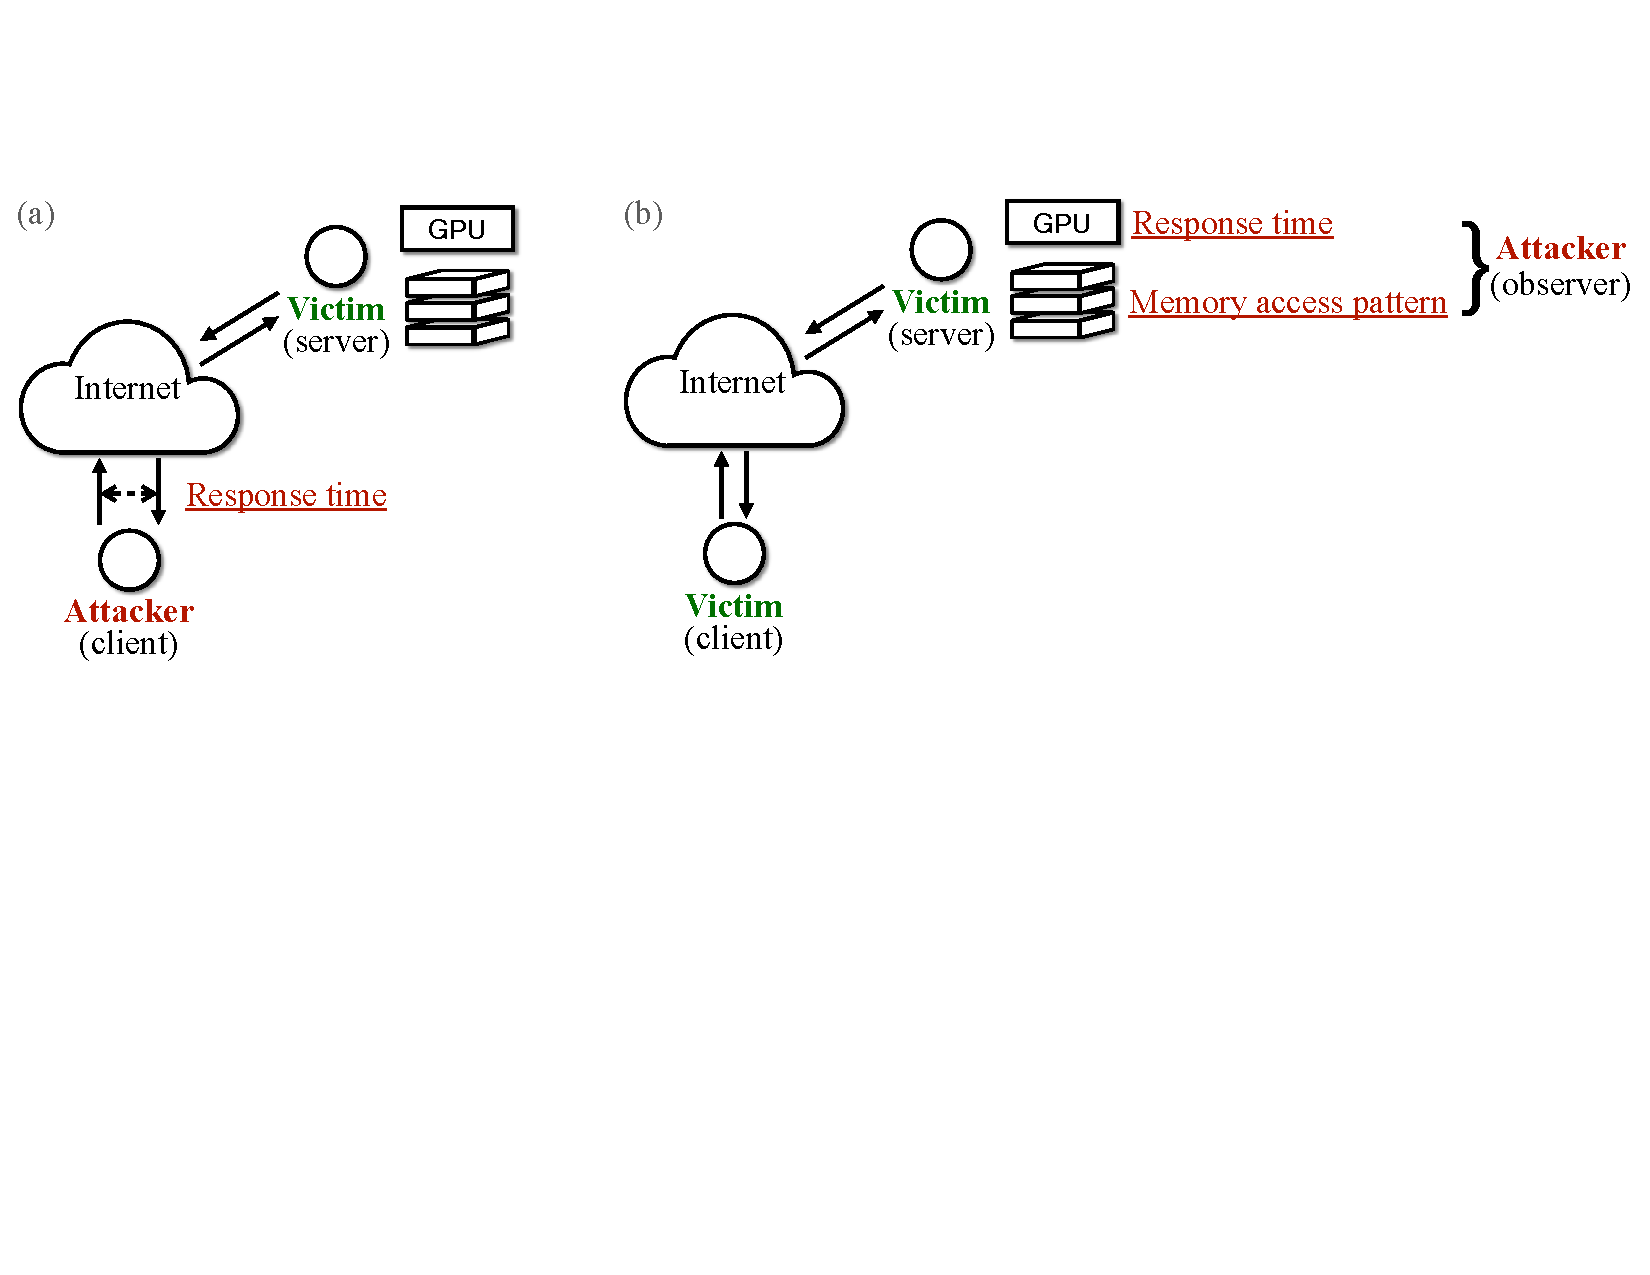
\includegraphics[clip,trim=0 10cm 0 2cm,width=0.72\pdfpagewidth]{figs/thrust1-fig.pdf}
    \caption{Attacker model considered in Thrust 1 \farzaneh{add quantitative?}}
    \label{fig:th1-attack}
    \end{figure}

\paragraph{Thrust 2. Active attacks}
In the attacks we consider in Thrust 2, the attacker has their own process in the cloud (as a client) which coexists with the victim process.
%
The victim and attacker both use the GPU server on the cloud and, through leaks caused by reuse of the registers and memory locations between processes, can gain access to the contents of the victim process's address space.
%
See Figure~\ref{fig:th2-attack}

\begin{figure}[h]
    \centering
    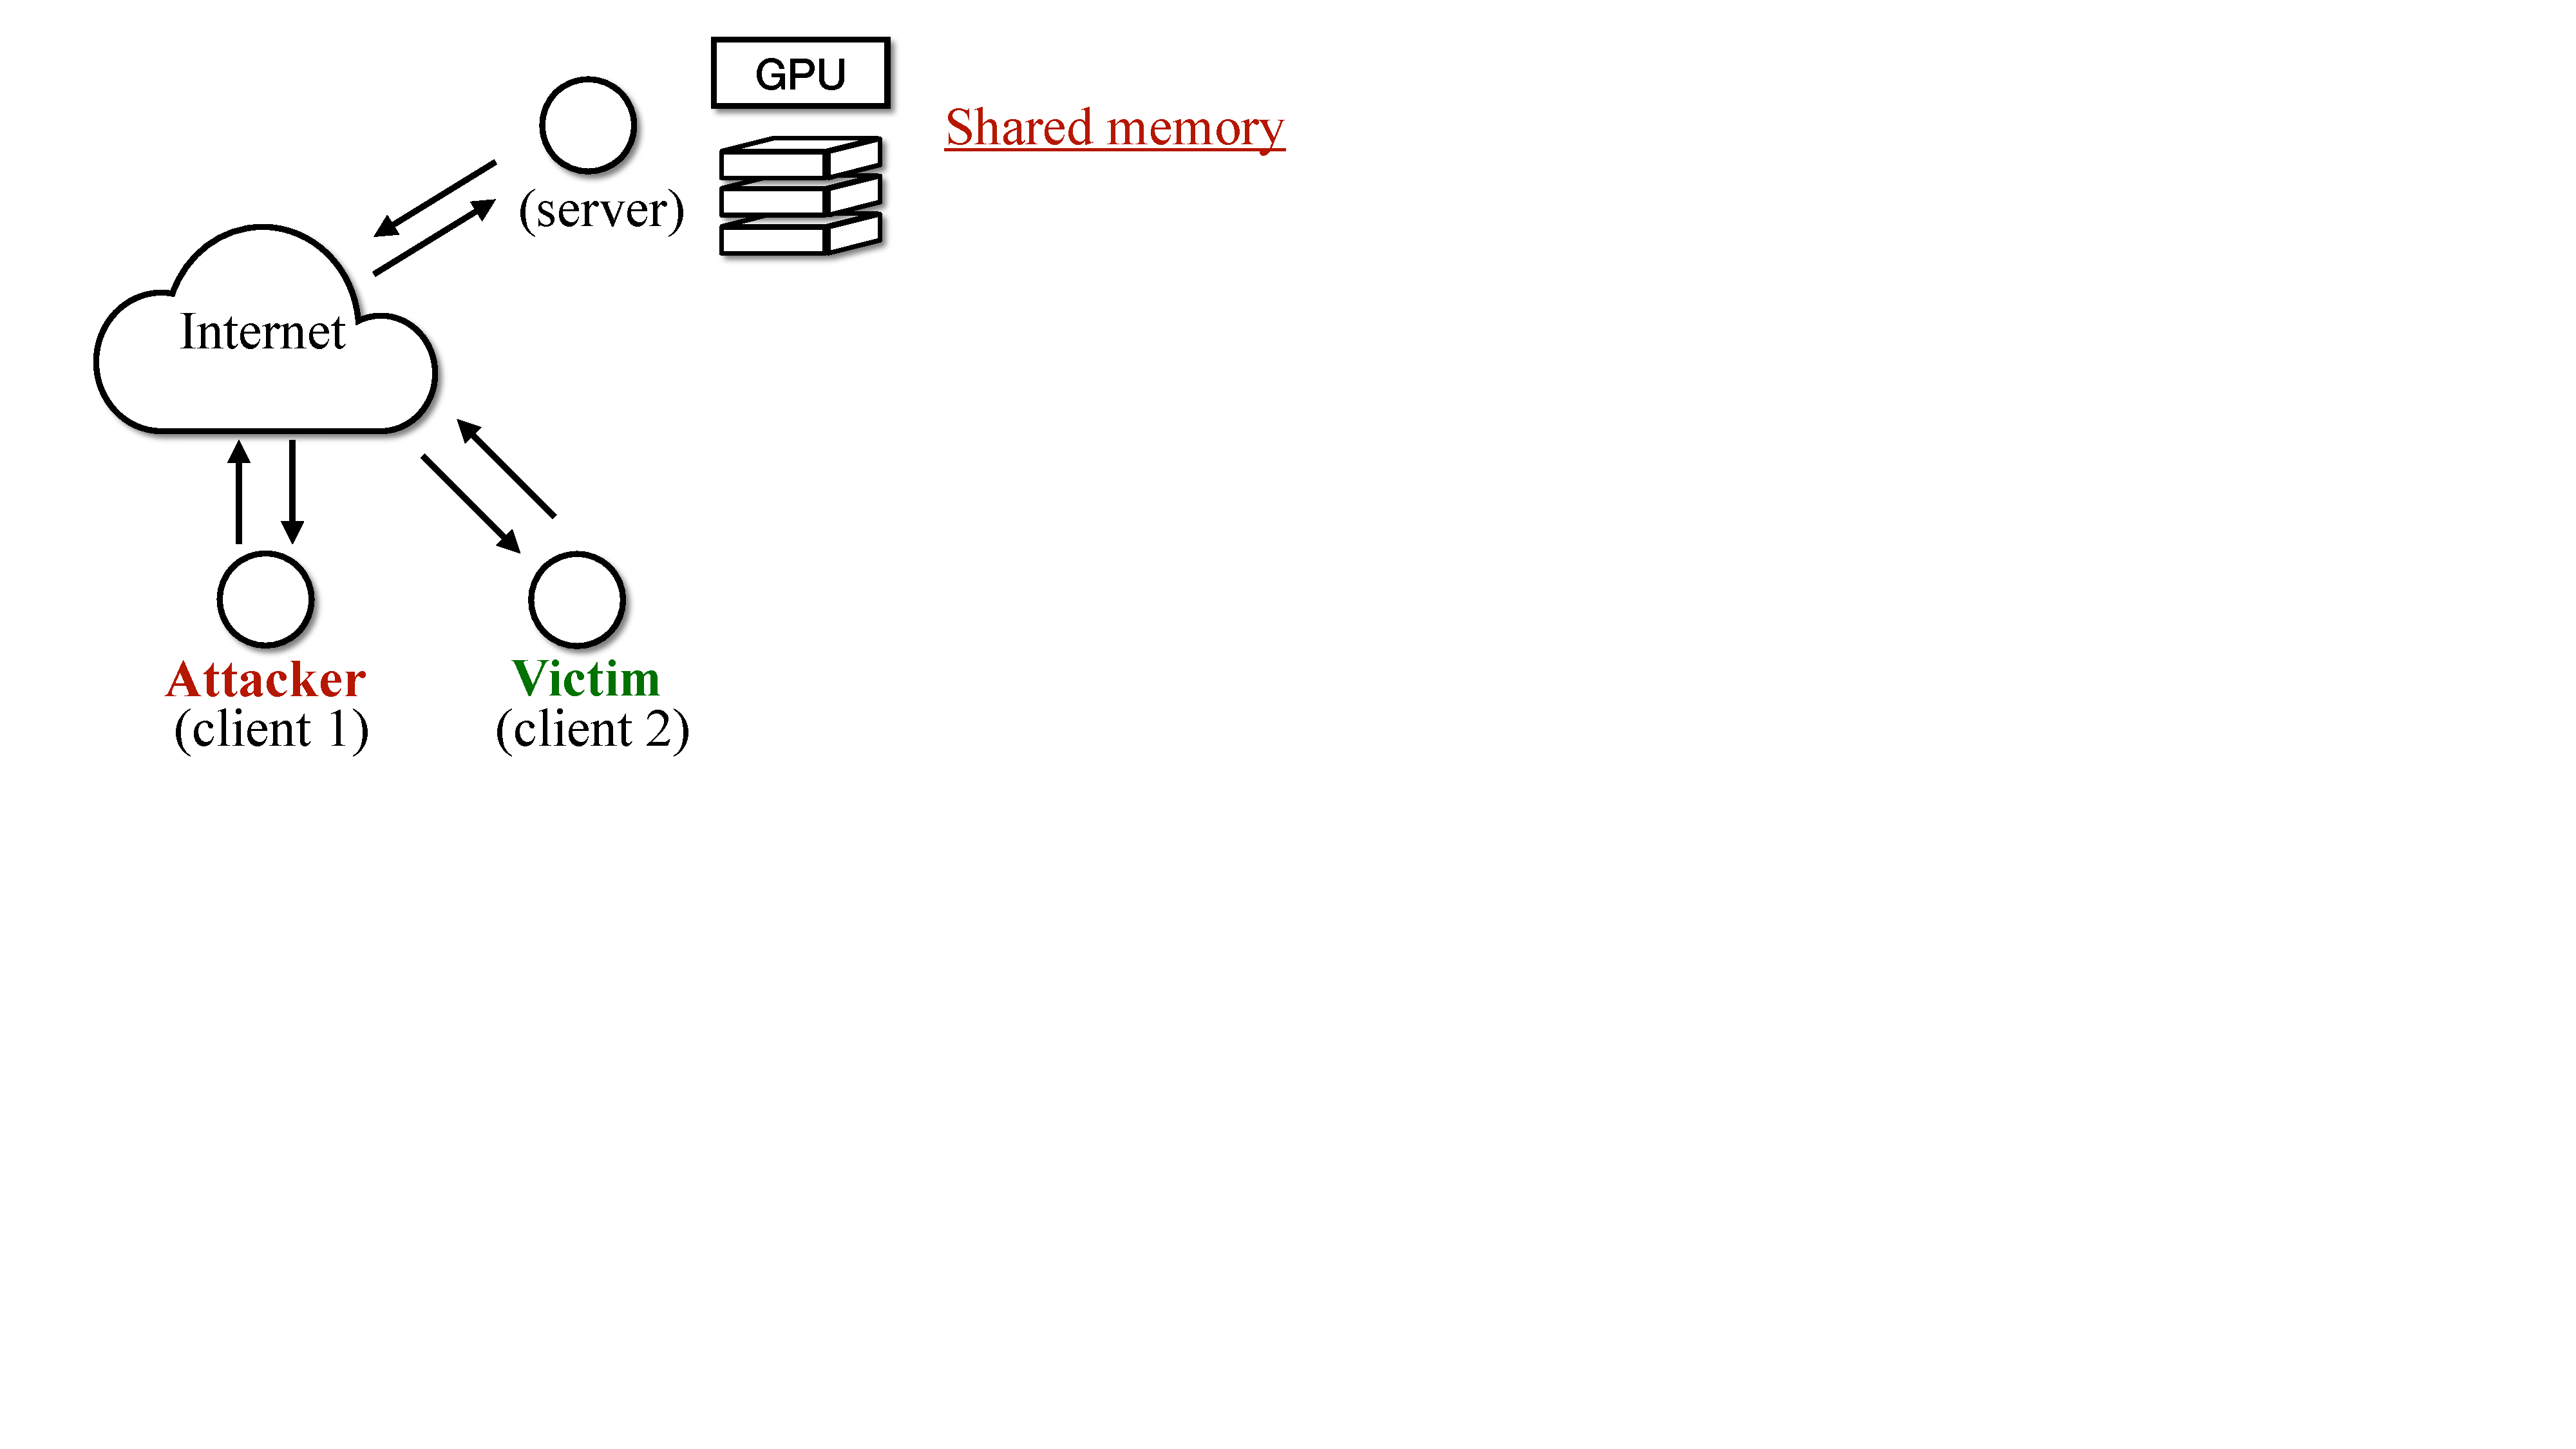
\includegraphics[clip,trim=0 17cm 10cm 0cm,width=0.72\pdfpagewidth]{figs/thrust2-fig.pdf}
    \caption{Attacker model considered in Thrust 2 \farzaneh{add more}}
    \label{fig:th2-attack}
    \end{figure}


\paragraph{Thrust 3. Case study}


In the first thrust we consider non-offensive attacks.
%
In the second thrust we consider offensive attacks.
%
We consider the unique parallelism paradigm in GPU as well as its memory behavior.

\paragraph{Related work on Modeling Execution Cost of CUDA.}
In prior NSF-supported work~\citep{MullerHo21}, PI Muller and his collaborator Jan Hoffmann developed MiniCUDA, a core calculus for CUDA with a formal dynamic semantics modelling the execution behavior of CUDA kernels on GPUs, including its cost of execution, taking into account factors such as bank conflicts and coalescing of global memory accesses.
%
The work also included a quantitative program logic for predicting the execution cost of a MiniCUDA kernel in terms of a provided {\em resource metric}, which can count any desired combination of bank conflicts, global memory transactions, and other features.
%
We plan to use MiniCUDA as the basis of our language model, and the semantics and quantitative program logic as a starting point for proving the soundness of our type system: our type system should guarantee that two runs of the kernel on states that differ only in high-security memory locations shouldn't differ in their observable execution behavior, including cost.
%
Muller and Hoffmann's implementation of the quantitative program logic, called RaCUDA, can also serve as a starting point for our implementation of the type system.

\paragraph{Related works on GPU security.}
(With a microbenchmark they measured the
time for a sequence of memory accesses of each thread in a block.)
%
The attack strategy commonly deployed in CPU-based. timing attack methods consist of one block of ciphertext, and profiling the associated time to process that
block. However, on a GPU it would be the encryption workload would contain multiblock messages, and on each data sample, the GPU
timing attackwould produce many blocks of ciphertext.
The key difference is that the GPU scenario will only
collect a single timing value for the multiple blocks.
Although many successful attack methods have been
demonstrated on CPU platforms, these methods cannot be directly applied to the GPU platform due to a
lack of accurate timing information and nondeterminism in thread scheduling.

\paragraph{Symbolic GPU security.}


